% Merged manuscript (paper1 + paper3) prepared for submission to the Journal of Medical Imaging (SPIE).
% DRAFT FOR AUTHOR REVIEW. Items marked TODO(author) must be resolved before submission.
%
% TODO(author): 1. Convert to the official SPIE journal LaTeX template (spiejour); this file uses the
%                  generic article class so it compiles anywhere.
% TODO(author): 2. Confirm JMI's abstract format (structured Purpose/Approach/Results/Conclusions assumed),
%                  length limit, and blind/non-blind review policy from the JMI author guidelines.
% TODO(author): 3. Add co-authors/supervisor (if any), email, funding, conflict-of-interest, ethics and
%                  data/code-availability statements.
% TODO(author): 4. The reference list (28 items) is thin for a journal article; add recent medical-imaging
%                  domain-shift, uncertainty and explainability literature. No references were invented here.
% TODO(author): 5. Confirm each table's source run (see Section "Note on run-to-run variation").
\documentclass[11pt]{article}
\usepackage[margin=1in]{geometry}
\usepackage{graphicx}
\usepackage{booktabs}
\usepackage{amsmath}
\usepackage{url}
\usepackage{setspace}
\onehalfspacing

\title{Trustworthiness Is Not One Property: Accuracy, Domain-Shift Robustness, Explainability, Abstention, and Deployment Cost in a Lightweight Cervical Cytology Screening Pipeline}
\author{Md Mostafizur Rahman\\
San Francisco Bay University, Fremont, California, USA\\
ORCID: 0009-0007-2022-8677}
\date{}

\begin{document}
\maketitle

\begin{abstract}
\noindent\textbf{Purpose.}
Lightweight vision transformers are proposed for automated cervical cytology screening, but ``trustworthy AI'' is usually evaluated as one property that a pipeline has or lacks. We test whether accuracy, domain-shift robustness, explainability, selective prediction, and deployment cost agree with each other on one cervical cytology pipeline.

\noindent\textbf{Approach.}
We benchmarked 12 CNN, full-size vision transformer, and efficient vision transformer models on SIPaKMeD, then evaluated all 12 zero-shot on three external cytology datasets (Herlev, Mendeley LBC, APCEM) harmonized to a binary normal/abnormal label. On a standard vision transformer, we compared three explainability methods against deletion/insertion faithfulness and expert-annotated nucleus boundaries, tested a combined confidence and conformal-set-size abstention rule, and measured parameters, FLOPs, CPU latency, and explanation cost.

\noindent\textbf{Results.}
The two smallest models (about 2.1M parameters) were the most accurate in distribution, but in-distribution accuracy did not predict robustness: the in-distribution leader ranked 10th of 12 on both Herlev and Mendeley LBC in the primary run, and on APCEM 9 of 12 models fell below chance AUROC. No measured static property predicted which model failed safely, and rankings changed across training seeds and datasets. Relevancy propagation was the most faithful explainability method on all three metrics and on a second backbone (nucleus concentration 2.71$\times$ chance versus 1.18$\times$ for attention rollout). Combining confidence with conformal set size helped only under severe shift (risk-coverage AUC 0.286 versus 0.324) and hurt in distribution and under mild shift. FLOPs did not predict CPU latency, and an explanation cost about 3.3$\times$ a bare prediction.

\noindent\textbf{Conclusions.}
Accuracy, robustness, explainability, abstention, and efficiency resolved differently on the same pipeline, so each needs its own test under the conditions of intended deployment.

\medskip
\noindent\textbf{Keywords:} cervical cytology, vision transformers, domain shift, explainability, selective prediction, conformal prediction, model efficiency
\end{abstract}

\section{Introduction}
\label{sec:intro}

Cervical cancer is substantially more curable when detected at a localized stage, yet access to screening is uneven across rural and urban U.S. counties, and specialist cytology capacity is limited in many settings. A growing literature proposes vision transformers, often marketed as efficient or lightweight variants, as classification backbones for automated cytology screening. Such a tool is only useful if it fails visibly rather than silently: a model that misclassifies confidently under conditions its training data did not cover is more dangerous than one that abstains.

``Trustworthy AI'' is usually evaluated as if it were a single property. In practice a screening pipeline makes at least five separable claims: (i) a lightweight model gives up little accuracy; (ii) its accuracy transfers across institutions, scanners, and staining protocols; (iii) its explanations are faithful; (iv) its confidence supports a reliable abstention rule; and (v) its efficiency claim holds under real measurement. A reader might reasonably assume that these resolve alike, so that testing one is enough. We test them side by side on one cervical cytology pipeline and ask whether they do.

We make four contributions.
\begin{enumerate}
\item \textbf{Efficiency--accuracy benchmark.} A 12-model benchmark on SIPaKMeD spanning CNN, full-size vision transformer, and efficient vision transformer families, in which the two most parameter-efficient models are also the most accurate in distribution.
\item \textbf{Domain-shift evaluation.} A zero-shot evaluation of all 12 models on three independently sourced external datasets (Herlev, Mendeley LBC, APCEM), together with a three-seed sensitivity check, showing that in-distribution accuracy, parameter count, FLOPs, and architecture family do not reliably predict which model fails safely, and that even apparent family-level patterns do not survive a third dataset or a change of seed.
\item \textbf{Explainability and abstention.} A comparison of relevancy propagation, attention rollout, and Grad-CAM against behavioral faithfulness and expert-annotated nucleus boundaries, replicated on a second backbone, and a test of whether combining temperature-scaled confidence with conformal prediction-set size improves selective prediction.
\item \textbf{Measured deployment cost.} A measurement of parameters, FLOPs, CPU latency, and explanation cost, showing that FLOPs do not predict latency and that returning an explanation costs roughly 3.3 times a bare prediction.
\end{enumerate}
The properties resolve differently: explainability method choice resolves cleanly, abstention composition resolves conditionally on shift severity, and robustness and efficiency resolve only under direct measurement. This divergence, rather than any single result, is the central finding, and it is visible only because the properties are tested jointly on one fixed pipeline.

\section{Related Work}
\label{sec:related}

\subsection{Efficient vision transformers}
Efficiency-oriented transformer variants fall into several loose lineages. Hybrid local--global designs (MobileViT \cite{mehta2022mobilevit}, MobileViTv2 \cite{mehta2022mobilevitv2}) interleave convolutional stages with transformer blocks. Distillation-oriented designs (DeiT \cite{touvron2021deit}) keep a standard ViT backbone \cite{dosovitskiy2021vit} but reach competitive accuracy with far less pretraining data. Hardware-aware designs (LeViT \cite{graham2021levit}, TinyViT \cite{wu2022tinyvit}) reintroduce convolutional stages to improve real-device latency rather than FLOP count alone. EfficientViT-M0 and EfficientViT-B0, the two smallest models in our registry, are often assumed to share a lineage because \texttt{timm} groups their tags; verified directly, they do not. EfficientViT-M0 uses cascaded group attention \cite{liu2023efficientvit}, whereas EfficientViT-B0 belongs to an unrelated lineage built on multi-scale linear attention for dense prediction \cite{cai2023efficientvit}. These design papers do not evaluate cross-institution domain shift as part of their efficiency claims, so efficiency and robustness are treated as unrelated properties.

\subsection{Domain shift and model selection in medical imaging}
A general medical-imaging literature documents that models selected on held-out in-distribution data can degrade under real distribution shift across scanners, sites, and populations, motivating external validation. That literature typically evaluates one or a few architectures. We instead sweep CNN, full-size transformer, and efficient transformer families at matched task and data scale and ask whether any measurable static model property predicts which model degrades least.

\subsection{Transformer explainability and faithfulness}
Attention rollout \cite{abnar2020quantifying} chains attention weights across layers as a relevance signal, a premise contested in the literature on whether attention is a faithful explanation. Relevancy propagation \cite{chefer2021transformer} weights each block's attention by its gradient with respect to the target class, making the map class-discriminative. Grad-CAM \cite{selvaraju2017gradcam} was designed for convolutional feature maps and is commonly adapted to transformers by targeting a block's token activations. Deletion/insertion faithfulness \cite{petsiuk2018rise} measures the effect of removing or revealing the regions an explanation marks as important on the model's own prediction. Evaluating localization against SIPaKMeD's expert-marked nucleus polygons avoids compounding the evaluation with a second model's errors.

\subsection{Selective prediction and calibration}
Temperature scaling \cite{guo2017calibration} calibrates confidence on a held-out split. Split conformal prediction gives a distribution-free coverage guarantee from a single calibration split, and its prediction-set size is a model-agnostic but coarse uncertainty proxy. MC Dropout \cite{gal2016dropout}, deep ensembles \cite{lakshminarayanan2017ensembles}, and evidential deep learning \cite{sensoy2018evidential} are alternative uncertainty signals that we do not evaluate here. To our knowledge, whether composing temperature-scaled confidence with conformal set size improves an abstention rule is not directly addressed by work that proposes either signal independently.

\subsection{Adjacent cervical and clinical-AI work}
Adjacent work includes a stacking-ensemble approach with explainable AI for cervical cancer diagnosis \cite{mohiuddin2025}, which we differ from by evaluating explainability against expert-annotated localization and behavioral faithfulness and by jointly evaluating efficiency and real cross-institution shift. A lightweight transformer with cross-scale attention and explainability for plant disease diagnosis \cite{rahman2026maizeformerx} motivates our treatment of efficiency and explainability as joint design goals, and two further papers address explainable clinical AI in other domains \cite{gony2026retinal,ahmed2026postsurgical}.

\section{Materials and Methods}
\label{sec:methods}

\subsection{Datasets}
\label{sec:datasets}
All models were trained on SIPaKMeD \cite{plissiti2018sipakmed}: 4,049 native-resolution single-cell crops derived from the dataset's own cytoplasm-polygon annotations, in five cytomorphology classes. External evaluation used Herlev \cite{jantzen2005herlev}, Mendeley LBC \cite{hussain2020mendeley}, and the APCEM-Enhanced Cervical Cytology Pap Smear Image Dataset \cite{aswini2026apcem} (4,253 images in the six-class Bethesda taxonomy: NILM, ASC-US, ASC-H, LSIL, HSIL, SSC). Because the four datasets use different label taxonomies, all were harmonized to one shared binary normal/abnormal label (for APCEM, NILM normal and all five atypical or dysplastic classes abnormal). The three external datasets differ from SIPaKMeD and from each other in acquisition pipeline, institution, and label granularity, so each is an independent test of generalization rather than a synthetic corruption of the same source images.

\subsection{Model registry}
\label{sec:registry}
Twelve models spanning three families were evaluated: CNN baselines (ResNet-50 \cite{he2016resnet}, MobileNetV2 \cite{sandler2018mobilenetv2}, EfficientNet-Lite0 \cite{tan2019efficientnet}); full-size vision transformers (ViT-Small \cite{dosovitskiy2021vit}, Swin-Tiny \cite{liu2021swin}); and efficient or mobile-oriented vision transformers (DeiT-Tiny \cite{touvron2021deit}, LeViT-128 \cite{graham2021levit}, TinyViT-5M \cite{wu2022tinyvit}, MobileViT-S \cite{mehta2022mobilevit}, MobileViTv2 \cite{mehta2022mobilevitv2}, EfficientViT-B0 \cite{cai2023efficientvit}, EfficientViT-M0 \cite{liu2023efficientvit}). All \texttt{timm} tags were verified against the pinned \texttt{timm} version, and the two EfficientViT variants' source papers were confirmed against \texttt{timm}'s model cards rather than inferred from the shared tag prefix.

\subsection{Training and in-distribution evaluation}
\label{sec:training}
Models were trained on SIPaKMeD with a 60/15/10/15 train/validation/calibration/test split, seed 13, a 30-epoch budget with early stopping (patience 7), on a single GPU. We report balanced accuracy, macro F1, AUROC, and parameter count. Evaluation stages were run as separate training and evaluation runs (see Section~\ref{sec:runvar}).

\subsection{Cross-dataset domain-shift evaluation}
\label{sec:shift}
Each model was evaluated zero-shot on Herlev, Mendeley LBC, and APCEM, with no retraining or recalibration, after label harmonization. To measure how much individual rankings depend on the training run, all 12 models were additionally retrained at two further seeds (17 and 29) and evaluated zero-shot on all three external datasets from a single checkpoint per model per seed.

\subsection{Explainability backbone and methods}
\label{sec:xai-methods}
Relevancy propagation and attention rollout are defined for standard multi-head self-attention blocks, and EfficientViT-M0 has no established propagation rule for either. Rather than force an ad hoc extension, the explainability and abstention experiments use \textbf{DeiT-Tiny}, a standard \texttt{timm} \texttt{VisionTransformer} that reached 0.9606 balanced accuracy in the benchmark (Section~\ref{sec:bench}), retrained for these experiments. All three methods produce a relevance map over the 14$\times$14 patch grid (224-pixel input, 16-pixel patches), upsampled to image resolution.
\emph{Attention rollout}: raw softmax attention averaged over heads and chained across all 12 blocks; class-agnostic.
\emph{Relevancy propagation}: the same rollout recurrence, with each block's contribution equal to $\mathrm{ReLU}(\nabla_{\text{attn}} \odot \text{attn})$ averaged over heads, where the gradient is taken with respect to the model's predicted-class logit; class-discriminative.
\emph{Grad-CAM (ViT-adapted)}: gradient-weighted channel importance applied to a transformer block's token activations. The target layer must be the \emph{second-to-last} block: DeiT-Tiny pools only the CLS token, so no layer after the final block mixes information back into patch positions. We verified this directly: every patch token's gradient at the last block's output was exactly zero, whereas the second-to-last block's patch-token gradients vary normally. Targeting the wrong block therefore yields an all-zero heatmap silently, not an error.

\subsection{Faithfulness and localization metrics}
\label{sec:xai-metrics}
\emph{Deletion/insertion AUC} \cite{petsiuk2018rise}: patches are ranked by a method's own relevance score and progressively replaced with (deletion) or revealed from (insertion) a heavily Gaussian-blurred copy of the image, tracking the predicted-class probability; we report the area under the probability-versus-fraction curve (lower is better for deletion, higher for insertion).
\emph{Nucleus concentration ratio}: SIPaKMeD provides expert-marked nucleus boundary polygons per cell, which we persist in crop-local pixel coordinates. The ratio is the fraction of a heatmap's total relevance mass inside the nucleus divided by the nucleus's share of image area. A ratio of 1.0 is exactly chance, and higher values mean relevance concentrates in the nucleus more than chance would predict, which is clinically the correct place to concentrate.

\subsection{Calibration, conformal prediction, and the combined abstention signal}
\label{sec:selective-methods}
Temperature scaling \cite{guo2017calibration} was fit on a calibration split disjoint from training and test data. Conformal prediction sets were built with a resampling-averaged split-conformal threshold. The combined selective-prediction signal rank-normalizes temperature-scaled max-softmax confidence and (inverted) conformal prediction-set size independently, then averages the ranks. Selective prediction was scored by risk-coverage AUC (lower is better) in distribution, on Herlev (moderate shift), and on Mendeley LBC (severe shift). The shift labels reflect the observed degradation of DeiT-Tiny on these datasets (Table~\ref{tab:shift12}).

\subsection{Efficiency and latency measurement}
\label{sec:eff-methods}
Parameters and FLOPs (via \texttt{torch.utils.flop\_counter.FlopCounterMode}, counting a multiply-add as two FLOPs) are architecture properties independent of trained weights, so they were measured without training. CPU latency (single-image batch, median of 30 iterations after 5 warm-up iterations) and memory (isolated per model in its own subprocess) were likewise measured with untrained weights, on one shared consumer laptop. The cost of an explanation was measured as a full forward, backward, and rollout pass for relevancy propagation's own predicted-class explanation against a bare forward pass, both on CPU. Robustness to synthetic degradation (JPEG compression, Gaussian blur, brightness/contrast shift at five severities each) and a synthetic out-of-distribution (OOD) sanity check (25 images of noise, solid colors, and checkerboards) were run on a freshly trained EfficientViT-M0.

\subsection{Note on run-to-run variation}
\label{sec:runvar}
In-distribution accuracy of the same model differs slightly between tables (for example, EfficientViT-M0: 0.9654 in Table~\ref{tab:bench}, 0.9737 in Table~\ref{tab:shift12}, 0.9621 in Table~\ref{tab:apcem}, and about 0.975 in the degradation experiment) because the evaluation stages were run as separate training and evaluation runs; at least the degradation experiment used a different random train/validation split. Comparisons are therefore valid within a table, not across tables. % TODO(author): confirm the cause for Tables 1, 2 and 3.

\section{Results}
\label{sec:results}

\subsection{Efficiency--accuracy benchmark}
\label{sec:bench}

\begin{table}[htbp]
\centering
\caption{In-distribution benchmark on SIPaKMeD, all 12 models, sorted by balanced accuracy (seed 13).}
\label{tab:bench}
\begin{tabular}{lrrrr}
\toprule
Model & Bal.\ acc. & Macro F1 & AUROC & Params \\
\midrule
\textbf{EfficientViT-M0} & \textbf{0.9654} & \textbf{0.9656} & 0.9985 & \textbf{2{,}157{,}401} \\
EfficientViT-B0 & 0.9623 & 0.9624 & 0.9983 & 2{,}135{,}413 \\
DeiT-Tiny & 0.9606 & 0.9607 & 0.9974 & 5{,}525{,}381 \\
Swin-Tiny & 0.9605 & 0.9606 & 0.9965 & 27{,}523{,}199 \\
TinyViT-5M & 0.9587 & 0.9589 & 0.9979 & 5{,}073{,}369 \\
MobileViT-S & 0.9570 & 0.9575 & 0.9979 & 4{,}940{,}837 \\
ResNet-50 & 0.9542 & 0.9540 & 0.9966 & 23{,}518{,}277 \\
LeViT-128 & 0.9458 & 0.9456 & 0.9946 & 8{,}447{,}786 \\
MobileViTv2 & 0.9387 & 0.9401 & 0.9966 & 4{,}391{,}406 \\
EfficientNet-Lite0 & 0.9375 & 0.9376 & 0.9944 & 3{,}377{,}413 \\
ViT-Small & 0.9374 & 0.9380 & 0.9960 & 21{,}667{,}589 \\
MobileNetV2 & 0.9357 & 0.9365 & 0.9952 & 2{,}230{,}277 \\
\bottomrule
\end{tabular}
\end{table}

The two smallest models in the registry were also the two most accurate (Table~\ref{tab:bench}, Fig.~\ref{fig:params-vs-acc}). EfficientViT-M0 exceeded the three large baselines, Swin-Tiny (27.5M parameters), ResNet-50 (23.5M), and ViT-Small (21.7M), by 0.5, 1.1, and 2.8 points of balanced accuracy respectively. On this task, at this data scale, the efficiency--accuracy trade-off does not appear in distribution. This is a single-seed result: the seed check in Section~\ref{sec:seeds} shows that the specific ordering at the top of Table~\ref{tab:bench} is not stable across seeds.

\begin{figure}[htbp]
\centering
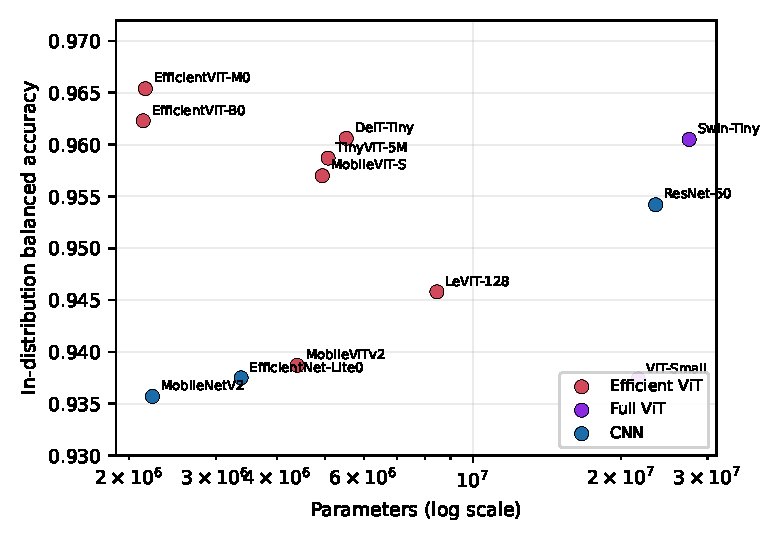
\includegraphics[width=0.82\textwidth]{figs/p1_fig1_params_vs_accuracy.pdf}
\caption{Parameters (log scale) versus in-distribution balanced accuracy, colored by architecture family. The two efficient-ViT models with the fewest parameters (EfficientViT-M0 and -B0) are also the two most accurate in this run.}
\label{fig:params-vs-acc}
\end{figure}

\subsection{Cross-dataset domain shift}
\label{sec:shiftresults}

\begin{table}[htbp]
\centering
\caption{Zero-shot balanced accuracy of all 12 models on Herlev and Mendeley LBC (binary normal/abnormal), seed 13, sorted by Mendeley LBC score. The SIPaKMeD column is in-distribution accuracy from the same run.}
\label{tab:shift12}
\small
\begin{tabular}{lrrr}
\toprule
Model (family, params) & SIPaKMeD & Herlev & Mendeley LBC \\
\midrule
EfficientNet-Lite0 (CNN, 3.38M) & 0.9455 & 0.5970 & \textbf{0.6674} \\
ResNet-50 (CNN, 23.5M) & 0.9556 & 0.6838 & 0.6082 \\
MobileViTv2 (eff.\ ViT, 4.39M) & 0.9638 & \textbf{0.7501} & 0.5418 \\
MobileNetV2 (CNN, 2.23M) & 0.9505 & 0.6919 & 0.5391 \\
DeiT-Tiny (eff.\ ViT, 5.5M) & 0.9504 & 0.7151 & 0.5230 \\
EfficientViT-B0 (eff.\ ViT, 2.14M) & 0.9738 & 0.6818 & 0.5217 \\
Swin-Tiny (full ViT, 27.5M) & 0.9590 & 0.7282 & 0.5192 \\
ViT-Small (full ViT, 21.7M) & 0.9573 & 0.7049 & 0.5084 \\
LeViT-128 (eff.\ ViT, 8.4M) & 0.9526 & 0.5777 & 0.4764 \\
EfficientViT-M0 (eff.\ ViT, 2.16M) & 0.9737 & 0.6716 & 0.4731 \\
TinyViT-5M (eff.\ ViT, 5.1M) & 0.9685 & 0.7327 & 0.4543 \\
MobileViT-S (eff.\ ViT, 4.94M) & 0.9520 & 0.7104 & \textbf{0.2927} (AUROC 0.215) \\
\bottomrule
\end{tabular}
\end{table}

\paragraph{In-distribution accuracy does not predict robustness.}
The two most accurate models in distribution in this run (EfficientViT-B0, 0.9738, and EfficientViT-M0, 0.9737) ranked 9th and 10th of 12 on Herlev and 6th and 10th of 12 on Mendeley LBC (Table~\ref{tab:shift12}). The comparison of EfficientViT-M0 with DeiT-Tiny is the sharpest case: the better in-distribution model (0.9737 versus 0.9504) was worse under both shifts (Herlev 0.6716 versus 0.7151; Mendeley LBC 0.4731 versus 0.5230, below the 0.50 chance floor). The same reversal appeared on APCEM (Table~\ref{tab:apcem}), where EfficientViT-M0 again scored lower under shift than DeiT-Tiny (0.3730 versus 0.4469) despite higher in-distribution accuracy (0.9621 versus 0.9589).

\paragraph{A family-level pattern appears on Mendeley LBC.}
All three CNNs scored 0.539--0.667, and eight of the nine transformer-family models scored 0.293--0.523. The ninth, MobileViTv2, scored 0.5418, above the lowest CNN (0.5391) by 0.003, a gap the seed check shows is noise (Section~\ref{sec:seeds}). The split does not hold on Herlev, where transformer models occupy both the best (MobileViTv2, TinyViT-5M) and the weakest (LeViT-128) positions.

\paragraph{Architecture lineage does not predict robustness.}
MobileViT-S collapsed on Mendeley LBC (balanced accuracy 0.2927, AUROC 0.215), meaning its predictions were anti-correlated with the ground truth, not merely uninformative. Its direct successor MobileViTv2 shows no such failure and was the strongest model in the registry on Herlev (0.7501).

\begin{figure}[htbp]
\centering
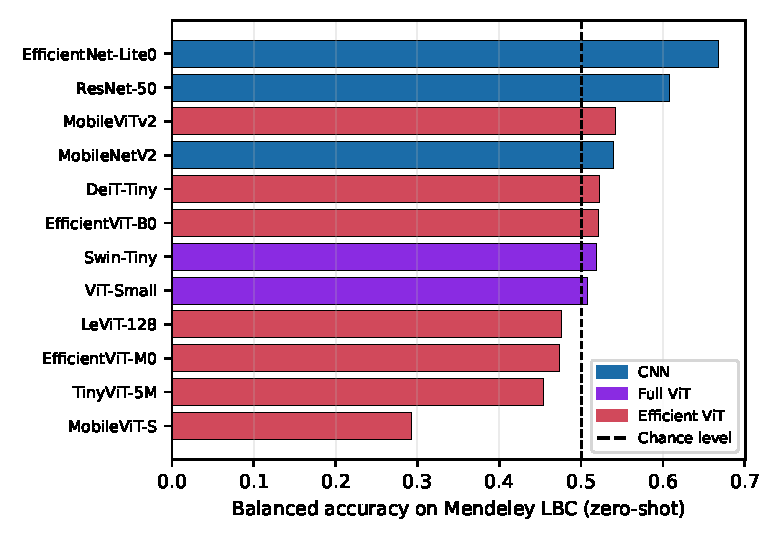
\includegraphics[width=0.82\textwidth]{figs/p1_fig2_mendeley_shift.pdf}
\caption{Balanced accuracy on Mendeley LBC (zero-shot), sorted and colored by architecture family. All three CNNs cluster above chance, and eight of nine transformer-family models cluster at or below chance, with MobileViT-S the sole catastrophic outlier.}
\label{fig:mendeley-shift}
\end{figure}

\begin{table}[htbp]
\centering
\caption{Zero-shot evaluation of all 12 models on APCEM, sorted by AUROC (this table comes from a separate training run; in-distribution accuracy differs from Table~\ref{tab:shift12}).}
\label{tab:apcem}
\small
\begin{tabular}{lrrr}
\toprule
Model (family, params) & SIPaKMeD & APCEM bal.\ acc. & APCEM AUROC \\
\midrule
MobileNetV2 (CNN, 2.23M) & 0.9623 & \textbf{0.6158} & \textbf{0.6528} \\
EfficientNet-Lite0 (CNN, 3.38M) & 0.9309 & 0.5393 & 0.5701 \\
LeViT-128 (eff.\ ViT, 8.4M) & 0.9001 & 0.5263 & 0.5376 \\
Swin-Tiny (full ViT, 27.5M) & 0.9330 & 0.4724 & 0.3082 \\
EfficientViT-B0 (eff.\ ViT, 2.14M) & 0.9638 & 0.4481 & 0.3206 \\
DeiT-Tiny (eff.\ ViT, 5.5M) & 0.9589 & 0.4469 & 0.3799 \\
MobileViTv2 (eff.\ ViT, 4.39M) & 0.9570 & 0.4290 & 0.4120 \\
TinyViT-5M (eff.\ ViT, 5.1M) & 0.9670 & 0.4100 & 0.3681 \\
EfficientViT-M0 (eff.\ ViT, 2.16M) & 0.9621 & 0.3730 & 0.3407 \\
MobileViT-S (eff.\ ViT, 4.94M) & 0.9687 & 0.3621 & 0.3161 \\
ViT-Small (full ViT, 21.7M) & 0.9538 & 0.3444 & 0.2555 \\
ResNet-50 (CNN, 23.5M) & 0.9639 & \textbf{0.3339} & 0.2929 \\
\bottomrule
\end{tabular}
\end{table}

\paragraph{A third dataset overturns the family-level pattern.}
On APCEM, 9 of 12 models fell below 0.50 on both balanced accuracy and AUROC (Table~\ref{tab:apcem}). Only MobileNetV2 (0.6158 balanced accuracy, AUROC 0.6528), EfficientNet-Lite0 (0.5393, 0.5701), and LeViT-128 (0.5263, 0.5376) scored above chance, and MobileNetV2 was the clear best. The CNN family spans both the best model (MobileNetV2) and the model with the lowest balanced accuracy (ResNet-50, 0.3339; AUROC 0.2929, second-lowest of the 12). The CNN-family robustness seen on Mendeley LBC therefore does not survive a third, independently sourced dataset.

\begin{figure}[htbp]
\centering
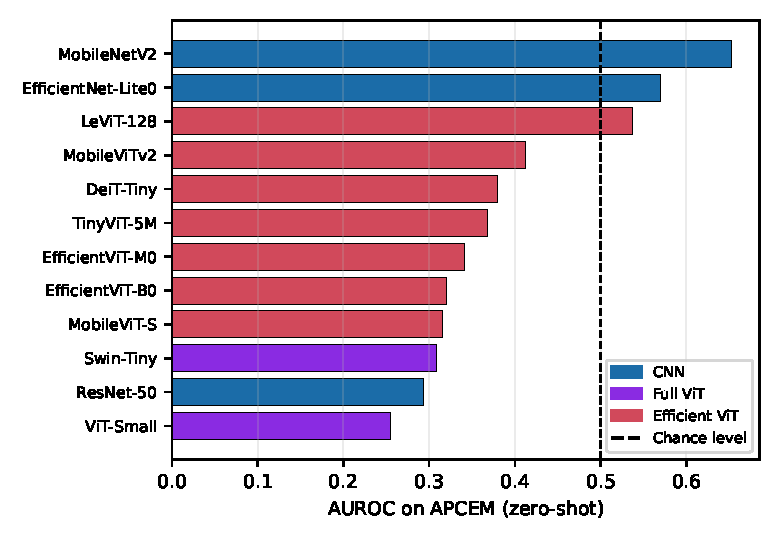
\includegraphics[width=0.82\textwidth]{figs/p1_fig3_apcem_shift.pdf}
\caption{AUROC on APCEM (zero-shot), sorted and colored by architecture family. Unlike Mendeley LBC, the CNN family spans both the best (MobileNetV2) and one of the worst (ResNet-50) models; no family-level pattern survives this third dataset.}
\label{fig:apcem-shift}
\end{figure}

\subsection{Seed sensitivity}
\label{sec:seeds}
Each headline model was trained once at seed 13. We measured seed-to-seed variance directly for two close-ranked pairs at two further seeds (17 and 29), and then extended the check to all 12 models on all three external datasets.

\paragraph{Close calls can go either way.}
On Mendeley LBC, MobileViTv2's 0.003 edge over MobileNetV2 (0.5418 versus 0.5391) does not survive: MobileNetV2 ranges 0.493--0.604 and MobileViTv2 ranges 0.494--0.623 across the three seeds, the ranges overlap almost completely, and the ranking flips at seed 17. On APCEM, EfficientViT-B0's 0.001 edge over DeiT-Tiny (0.4481 versus 0.4469) does survive: EfficientViT-B0 ranges 0.421--0.448, DeiT-Tiny ranges 0.367--0.447, EfficientViT-B0 wins at all three seeds, and its margin widens (to 0.027, then 0.067). The same kind of close call produced opposite outcomes once tested.

\paragraph{The Mendeley LBC family split is seed-specific.}
At seed 13 only 1 of 9 transformer-family models exceeds the weakest CNN (by 0.003). At seed 17, 3 of 9 do, and at seed 29, 4 of 9 do, by margins up to 0.11.

\paragraph{The in-distribution leader is not reliably the robustness loser.}
EfficientViT-M0 is the (near-)in-distribution leader and ranks 10th of 12 on both Herlev and Mendeley LBC at seed 13. At seed 29 it is the outright in-distribution winner and mid-pack under shift on both datasets (rank 4--5 of 12), and at seed 17 it is not even the in-distribution winner (rank 10 of 12). It should be read as a seed-13 illustration rather than a reproducible property of that model. The general claim it illustrates, that no static property predicts shift robustness, is unaffected, and a poster-child example that itself varies by seed is one more demonstration of that unreliability.

\paragraph{Some findings replicate cleanly.}
Herlev's inverse pattern (most transformer models outscoring the CNNs) and MobileNetV2's status as the strongest model on APCEM both replicate across all three seeds.

\subsection{Explainability fidelity}
\label{sec:xai-results}

\begin{table}[htbp]
\centering
\caption{Explainability method comparison on DeiT-Tiny, 50 SIPaKMeD test images (10 per class), all matched to a real nucleus polygon.}
\label{tab:xai}
\begin{tabular}{lrrr}
\toprule
Method & Deletion AUC$\downarrow$ & Insertion AUC$\uparrow$ & Nucleus conc.$\uparrow$ \\
\midrule
\textbf{Relevancy propagation} & \textbf{0.734} & \textbf{0.970} & \textbf{2.714} \\
Grad-CAM (ViT-adapted) & 0.818 & 0.877 & 1.472 \\
Attention rollout & 0.825 & 0.936 & 1.177 \\
\bottomrule
\end{tabular}
\end{table}

\begin{figure}[htbp]
\centering
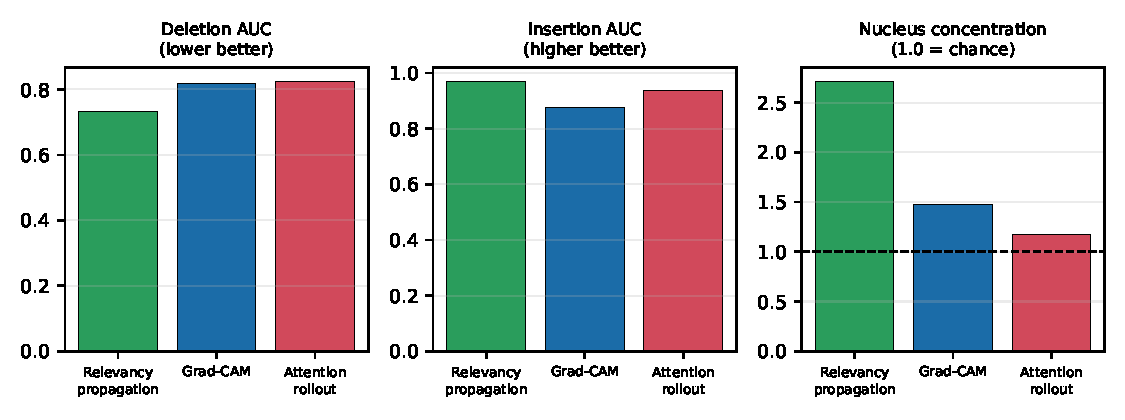
\includegraphics[width=\textwidth]{figs/p3_fig1_explainability_metrics.pdf}
\caption{Deletion AUC, insertion AUC, and nucleus concentration ratio for the three explainability methods. Relevancy propagation wins on all three, with the widest margin on nucleus concentration.}
\label{fig:xai-metrics}
\end{figure}

Relevancy propagation won every comparison (Table~\ref{tab:xai}), by a wide margin on nucleus concentration (2.71 times chance versus attention rollout's 1.18 times, barely above chance). We attribute this to a mechanistic difference rather than noise: attention rollout is class-agnostic, a disadvantage on an inherently class-discriminative test, whereas relevancy propagation is class-discriminative and integrates the gradient-weighted signal across all twelve blocks.

\paragraph{Second backbone.}
This single-backbone result rested on DeiT-Tiny, so we repeated the comparison on ViT-Small, a structurally identical \texttt{VisionTransformer} (same \texttt{global\_pool="token"}, \texttt{num\_prefix\_tokens=1}, 12 blocks, verified directly), trained fresh with the same recipe and seed.

\begin{table}[htbp]
\centering
\caption{Explainability ranking on a second backbone (ViT-Small) versus the original (DeiT-Tiny).}
\label{tab:xai-vits}
\small
\begin{tabular}{lrrrrrr}
\toprule
 & \multicolumn{3}{c}{DeiT-Tiny (original)} & \multicolumn{3}{c}{ViT-Small (2nd backbone)} \\
Method & Del.$\downarrow$ & Ins.$\uparrow$ & Conc.$\uparrow$ & Del.$\downarrow$ & Ins.$\uparrow$ & Conc.$\uparrow$ \\
\midrule
\textbf{Relevancy prop.} & \textbf{0.734} & \textbf{0.970} & \textbf{2.71} & \textbf{0.816} & \textbf{0.965} & \textbf{4.20} \\
Grad-CAM & 0.818 & 0.877 & 1.47 & 0.888 & 0.895 & 1.35 \\
Attn.\ rollout & 0.825 & 0.936 & 1.18 & 0.888 & 0.927 & 0.97 \\
\bottomrule
\end{tabular}
\end{table}

The ranking replicated exactly (Table~\ref{tab:xai-vits}): relevancy propagation wins all three metrics on ViT-Small, with an even wider nucleus-concentration margin (4.20 times chance versus its closest competitor's 1.35 times). The claim is scoped deliberately. Both backbones are pure multi-head self-attention transformers of different widths and depths, not different architecture families, and whether the ranking survives a hybrid convolution--attention backbone remains untested because relevancy propagation is not defined for EfficientViT-M0's architecture.

\subsection{Selective prediction}
\label{sec:selective-results}
Two proposed sub-claims about safe composition hold by construction in our post-hoc-attachment architecture and were verified rather than assumed: temperature scaling changed zero argmax predictions on the calibration split, and explanation computation is a read-only analysis that cannot alter model weights.

\begin{table}[htbp]
\centering
\caption{Selective-prediction risk-coverage AUC (lower is better) on DeiT-Tiny: confidence alone, conformal set size alone, and the combined signal.}
\label{tab:selective}
\begin{tabular}{lrrr}
\toprule
Condition & Confidence only & Set size only & Combined \\
\midrule
In-distribution & \textbf{0.0050} & 0.0834 & 0.0173 \\
Herlev (moderate shift) & \textbf{0.1190} & 0.3281 & 0.1793 \\
Mendeley LBC (severe shift) & 0.3244 & 0.4395 & \textbf{0.2855} \\
\bottomrule
\end{tabular}
\end{table}

\begin{figure}[htbp]
\centering
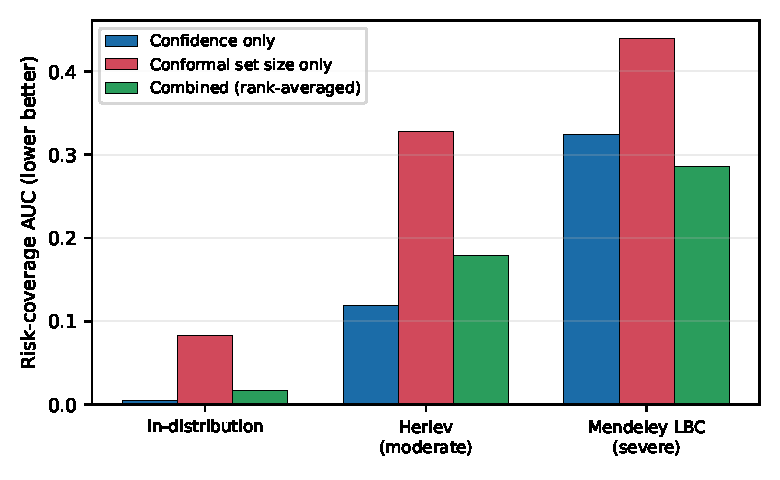
\includegraphics[width=0.85\textwidth]{figs/p3_fig3_combined_selective.pdf}
\caption{Risk-coverage AUC for confidence alone, conformal set size alone, and the rank-averaged combination at three conditions. Combining hurts in distribution and under moderate shift but helps under severe shift.}
\label{fig:combined-selective}
\end{figure}

Composition is not a uniform win (Table~\ref{tab:selective}). In distribution and under moderate shift, confidence alone is already the best individual signal, and combining it with the noisier, discrete conformal-set-size signal dilutes it. Under severe shift the combined signal is the best of the three, beating confidence alone (0.2855 versus 0.3244). Combining therefore helps exactly where the better individual signal was already struggling and hurts elsewhere, so an evaluation at one shift severity would report the result backwards. Even the best signal remains far from a safe abstention rule under severe shift. This conclusion rests on one backbone (DeiT-Tiny).

\subsection{Resource efficiency and deployment cost}
\label{sec:eff-results}

\begin{table}[htbp]
\centering
\caption{Parameters, FLOPs (multiply-add counted as 2), and median single-image CPU latency for all 12 models (untrained weights, one shared consumer laptop).}
\label{tab:eff}
\small
\begin{tabular}{lrrr}
\toprule
Model & Params & FLOPs (G) & CPU latency (ms) \\
\midrule
EfficientViT-M0 & 2{,}157{,}401 & 0.158 & 36.2 \\
EfficientViT-B0 & 2{,}135{,}413 & 0.198 & 41.6 \\
MobileNetV2 & 2{,}230{,}277 & 0.599 & 33.5 \\
EfficientNet-Lite0 & 3{,}377{,}413 & 0.768 & \textbf{137.7} \\
LeViT-128 & 8{,}447{,}786 & 0.809 & 17.5 \\
DeiT-Tiny & 5{,}525{,}381 & 2.149 & \textbf{15.4} \\
TinyViT-5M & 5{,}073{,}369 & 2.510 & 44.9 \\
MobileViT-S & 4{,}940{,}837 & 3.645 & 66.3 \\
MobileViTv2 & 4{,}391{,}406 & 3.623 & 65.2 \\
ResNet-50 & 23{,}518{,}277 & 8.174 & 32.0 \\
ViT-Small & 21{,}667{,}589 & 8.482 & 26.8 \\
Swin-Tiny & 27{,}523{,}199 & 8.980 & 54.0 \\
\bottomrule
\end{tabular}
\end{table}

Neither parameter count nor FLOPs reliably predicted CPU latency (Table~\ref{tab:eff}). EfficientNet-Lite0 (3.38M parameters, 0.77 GFLOPs) had more than four times ResNet-50's latency (137.7 ms versus 32.0 ms) despite ResNet-50 having roughly ten times the FLOPs. The two ``Mobile''-branded transformers had the highest transformer-family latency (66.3 and 65.2 ms) despite 3.6 GFLOPs, well below Swin-Tiny's 9.0 GFLOPs at 54.0 ms. EfficientViT-M0, the leader on parameters and FLOPs, was not the fastest model in wall-clock terms: DeiT-Tiny (15.4 ms) and LeViT-128 (17.5 ms) were both faster despite having about 14 and 5 times more FLOPs respectively. Repeating the EfficientViT-M0 measurement in isolation three times gave 27.4, 28.4, and 27.9 ms, against 28.3 and 36.2 ms in two full sweeps, so individual latencies carry roughly a 30\% run-to-run swing from background load. The relative ordering (EfficientNet-Lite0 far slower than all others, DeiT-Tiny and LeViT-128 fastest) was stable across repeated runs.

\paragraph{Cost of an explanation.}
On CPU, a bare DeiT-Tiny forward pass had a median latency of 49.6 ms, and a prediction that also returned a relevancy-propagation explanation cost 164.1 ms, about 3.3 times the bare-prediction cost. This pair was measured in the explanation-cost experiment and is not directly comparable with the 15.4 ms in Table~\ref{tab:eff}, which came from a separate full-registry sweep. % TODO(author): confirm why the two DeiT-Tiny CPU latencies (15.4 ms and 49.6 ms) differ (batch, load, trained vs untrained, or a different measurement protocol).

\paragraph{Synthetic degradation and OOD check.}
EfficientViT-M0 degraded gradually, not catastrophically, under all three corruptions (Fig.~\ref{fig:degradation}). Gaussian blur was by far the most damaging, costing 32.8 points of balanced accuracy at its most severe level (radius 8), roughly double JPEG compression's worst case (15.5 points) and nearly double brightness/contrast's (18.1 points). A plausible reason is that Bethesda-system diagnosis depends on fine nuclear texture, which blur removes directly. On the 25-image synthetic OOD sample, mean max-softmax confidence fell from 0.985 (real in-distribution images) to 0.743, a real drop but far above the 0.20 chance level for this five-class task, so confidence thresholding alone gives only a weak OOD signal.

\begin{figure}[htbp]
\centering
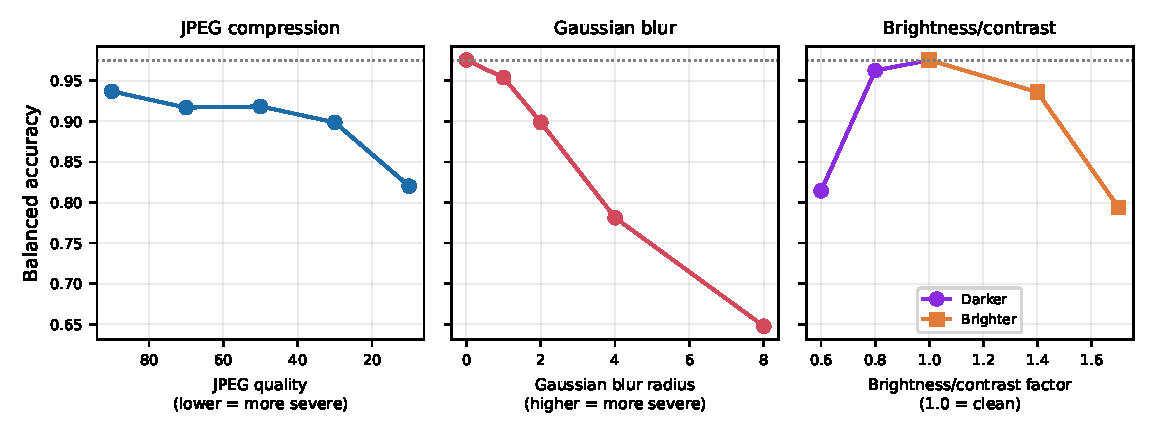
\includegraphics[width=\textwidth]{figs/p3_fig2_degradation_curves.pdf}
\caption{Balanced accuracy versus corruption severity for three synthetic degradations (EfficientViT-M0, SIPaKMeD test set). The dotted line marks the clean baseline (0.975). Gaussian blur causes the steepest decline.}
\label{fig:degradation}
\end{figure}

\section{Discussion}
\label{sec:discussion}

Read together, the results argue against several intuitive heuristics for selecting and verifying a deployment pipeline from a single evaluation. \emph{``Smaller is worse''} is falsified in distribution (Section~\ref{sec:bench}). \emph{``The in-distribution leader is the safe choice''} is falsified by the leader's poor ranks under shift in the primary run, and by the fact that even this ranking varies with the training seed (Section~\ref{sec:seeds}). \emph{``Architecture lineage predicts robustness''} is falsified by MobileViT-S and MobileViTv2, which share a lineage and produced a catastrophic failure and a top result on the same evaluation. \emph{``CNNs are the robust family''} looked stable on Herlev and Mendeley LBC, but a third, independently sourced dataset (APCEM) overturned it, and a seed check showed that the Mendeley LBC split was itself seed-specific. The sharpest methodological point is that a robustness pattern that survives two external datasets is not guaranteed to survive a third, so ``tested under two external shifts'' is not a licence to stop testing.

The other three properties behaved differently from robustness and from each other. Explainability method choice produced the cleanest result, a single winner on every metric and on a second backbone, so that choosing the method is a reliably beneficial engineering decision in this setting. Abstention composition was conditional on shift severity. Efficiency claims required direct measurement: FLOPs did not predict latency, an explanation cost about 3.3 times a bare prediction, and OOD confidence dropped only partially. No single verification strategy (pick the best method once, assume composition helps, trust an architectural efficiency claim) would have characterized all five properties correctly.

For deployment, the practical implications are direct. A backbone should not be chosen from an in-distribution leaderboard, however carefully measured, and robustness must be measured under the shift the deployment will actually face, ideally across multiple seeds. Confidence-based abstention, even when combined with conformal set size, did not reach a reliable operating point under severe shift, so a screening tool should expect to route a substantial fraction of shifted-domain cases to specialist review. Blur is the most damaging of the tested corruptions, which makes focus quality in any handheld or low-cost capture setting a first priority for field validation.

\section{Limitations}
\label{sec:limitations}

\textbf{Data.} All four datasets come from a small number of source institutions, and the three external shifts are real cross-institution shifts, not a systematic sweep of shift types (scanner resolution, stain intensity, or demographics varied independently). The findings are demonstrated for these three shifts, and only the higher-level conclusion, that no static property reliably predicts robustness, is expected to generalize; specific rankings, including which model is most robust, should not be assumed to transfer to a fourth dataset. Label harmonization to a binary task discards clinically important granularity. SIPaKMeD (about 4,000 images) is a single-institution training source.

\textbf{Seeds and runs.} Each headline result is a single train/validation/calibration/test split at seed 13. Seed variance was measured for all 12 models at two further seeds, and it showed that several single-model and single-dataset claims are seed-specific (the Mendeley LBC family split and EfficientViT-M0 as the in-distribution winner that fails under shift), so individual rows and close-ranked comparisons should be read with caution. The higher-level conclusions do not rest on any single seed-fragile comparison. Different tables come from separate runs (Section~\ref{sec:runvar}). No trained-weight checkpoints persisted, so reproducing a row means retraining from scratch with the released code.

\textbf{Backbone mismatch.} The explainability and abstention experiments use DeiT-Tiny, not the benchmark's in-distribution leader, because relevancy propagation is not defined for EfficientViT-M0. The explainability ranking was confirmed on one additional same-family backbone (ViT-Small), but the abstention-composition result and the degradation and OOD findings were not re-tested on it. Whether any of these results transfer to a hybrid convolution--attention backbone, or to a different imaging task, is untested.

\textbf{Measurement.} The explainability comparison uses 50 test images from one fixed stratified sample; a different sample could shift the exact values, although the winning margins are large. The OOD check uses a small synthetic sample (25 images) rather than a natural out-of-domain dataset. CPU latency was measured on one shared consumer laptop (about 30\% run-to-run swing) rather than dedicated or clinic-grade hardware, so the 3.3 times explanation-cost multiplier should be read as approximate. Accuracy, macro F1, and AUROC are standard metrics, which reduces the risk that the findings are artifacts of an unusual metric.

\textbf{Clinical validity.} No clinical or expert-review validation of explanation fidelity was performed. Agreement with a nucleus boundary is not equivalent to a cytotechnologist judging an explanation clinically meaningful. No prospective or reader-study evaluation of the full pipeline was performed.

\section{Conclusion}
\label{sec:conclusion}

Five properties of one cervical cytology screening pipeline, tested together, did not resolve alike. Parameter-efficient vision transformers did not trade accuracy for efficiency in distribution, yet the in-distribution leaderboard misled about robustness: no static property we measured predicted which model fails safely, and even apparent family-level patterns did not survive a third external dataset or a change of training seed. Relevancy propagation was a clearly better explainability method than attention rollout or Grad-CAM, on behavioral faithfulness and on expert-annotated localization, and the ranking replicated on a second backbone. Combining two uncertainty signals for abstention helped only under the severe shift where the better individual signal was already failing. Efficiency claims held only under direct measurement, since FLOPs did not predict latency and an explanation cost roughly 3.3 times a bare prediction. Each property needed its own test, on its own terms, under the conditions of intended deployment.

\section*{Disclosures}
% TODO(author): add conflict-of-interest, funding, ethics, data availability and code availability statements.
The authors declare no conflicts of interest. % TODO(author): confirm.

\begin{thebibliography}{99}

\bibitem{plissiti2018sipakmed}
Plissiti, M.E., Dimitrakopoulos, P., Sfikas, G., Nikou, C., Krikoni, O., Charchanti, A.: SIPAKMED: A new dataset for feature and image based classification of normal and pathological cervical cells in Pap smear images. In: 2018 IEEE International Conference on Image Processing (ICIP), pp.\ 3144--3148 (2018)

\bibitem{he2016resnet}
He, K., Zhang, X., Ren, S., Sun, J.: Deep residual learning for image recognition. In: CVPR (2016)

\bibitem{sandler2018mobilenetv2}
Sandler, M., Howard, A., Zhu, M., Zhmoginov, A., Chen, L.C.: MobileNetV2: Inverted residuals and linear bottlenecks. In: CVPR (2018)

\bibitem{tan2019efficientnet}
Tan, M., Le, Q.: EfficientNet: Rethinking model scaling for convolutional neural networks. In: ICML (2019)

\bibitem{dosovitskiy2021vit}
Dosovitskiy, A., et al.: An image is worth 16x16 words: Transformers for image recognition at scale. In: ICLR (2021)

\bibitem{liu2021swin}
Liu, Z., Lin, Y., Cao, Y., Hu, H., Wei, Y., Zhang, Z., Lin, S., Guo, B.: Swin Transformer: Hierarchical vision transformer using shifted windows. In: ICCV (2021)

\bibitem{touvron2021deit}
Touvron, H., Cord, M., Douze, M., Massa, F., Sablayrolles, A., J\'egou, H.: Training data-efficient image transformers \& distillation through attention. In: ICML (2021)

\bibitem{graham2021levit}
Graham, B., El-Nouby, A., Touvron, H., Stock, P., Joulin, A., J\'egou, H., Douze, M.: LeViT: a vision transformer in ConvNet's clothing for faster inference. In: ICCV (2021)

\bibitem{wu2022tinyvit}
Wu, K., et al.: TinyViT: Fast pretraining distillation for small vision transformers. In: ECCV (2022)

\bibitem{mehta2022mobilevit}
Mehta, S., Rastegari, M.: MobileViT: Light-weight, general-purpose, and mobile-friendly vision transformer. In: ICLR (2022)

\bibitem{mehta2022mobilevitv2}
Mehta, S., Rastegari, M.: Separable self-attention for mobile vision transformers. arXiv preprint (2022)

\bibitem{cai2023efficientvit}
Cai, H., Li, J., Hu, M., Gan, C., Han, S.: EfficientViT: Multi-scale linear attention for high-resolution dense prediction. In: ICCV (2023)

\bibitem{liu2023efficientvit}
Liu, X., Peng, H., Zheng, N., Yang, Y., Hu, H., Yuan, Y.: EfficientViT: Memory efficient vision transformer with cascaded group attention. In: CVPR (2023)

\bibitem{jantzen2005herlev}
Jantzen, J., Norup, J., Dounias, G., Bjerregaard, B.: Pap-smear benchmark data for pattern classification. In: Proceedings of Nature Inspired Smart Information Systems (NiSIS), pp.\ 1--9 (2005)

\bibitem{hussain2020mendeley}
Hussain, E., Mahanta, L.B., Borah, H., Das, C.R.: Liquid based-cytology Pap smear dataset for automated multi-class diagnosis of pre-cancerous and cervical cancer lesions. Data in Brief 30, 105589 (2020)

\bibitem{aswini2026apcem}
Aswini, H.: APCEM-Enhanced Cervical Cytology Image Dataset (Version 2) [Data set]. Mendeley Data (2026). \url{https://doi.org/10.17632/snzb5g6ddy.2}

\bibitem{chefer2021transformer}
Chefer, H., Gur, S., Wolf, L.: Transformer interpretability beyond attention visualization. In: CVPR (2021)

\bibitem{abnar2020quantifying}
Abnar, S., Zuidema, W.: Quantifying attention flow in transformers. In: ACL (2020)

\bibitem{selvaraju2017gradcam}
Selvaraju, R.R., Cogswell, M., Das, A., Vedantam, R., Parikh, D., Batra, D.: Grad-CAM: Visual explanations from deep networks via gradient-based localization. In: ICCV (2017)

\bibitem{gal2016dropout}
Gal, Y., Ghahramani, Z.: Dropout as a Bayesian approximation: Representing model uncertainty in deep learning. In: ICML (2016)

\bibitem{lakshminarayanan2017ensembles}
Lakshminarayanan, B., Pritzel, A., Blundell, C.: Simple and scalable predictive uncertainty estimation using deep ensembles. In: NeurIPS (2017)

\bibitem{sensoy2018evidential}
Sensoy, M., Kaplan, L., Kandemir, M.: Evidential deep learning to quantify classification uncertainty. In: NeurIPS (2018)

\bibitem{petsiuk2018rise}
Petsiuk, V., Das, A., Saenko, K.: RISE: Randomized input sampling for explanation of black-box models. In: BMVC (2018)

\bibitem{guo2017calibration}
Guo, C., Pleiss, G., Sun, Y., Weinberger, K.Q.: On calibration of modern neural networks. In: ICML (2017)

\bibitem{mohiuddin2025}
Mohiuddin, A.B., Rahman, M.M., et al.: Accelerated and accurate cervical cancer diagnosis using a novel stacking ensemble method with explainable AI. In: International Conference on Quantum Photonics, Artificial Intelligence (2025)

\bibitem{rahman2026maizeformerx}
Rahman, M.M., et al.: MaizeFormerX: a lightweight vision transformer with cross-scale attention for explainable maize leaf disease diagnosis. Scientific Reports (2026)

\bibitem{gony2026retinal}
Gony, M.N., Shuvra, S.M.K., Poudel, R., Dhakal, K., Rahman, M.M., et al.: Dual-view semi-supervised retinal disease recognition via chromatic structural decomposition and cross-view contrastive learning. In: International Conference on Power, Electronics, Communications (2026)

\bibitem{ahmed2026postsurgical}
Ahmed, M., Ahmed, F., Mow, S.M., Taha, P.A., Barua, S., Rahman, M.M., et al.: An explainable multimodal AI framework with reinforcement learning for post-surgical clinical decision support. medRxiv (2026)

\end{thebibliography}
\end{document}
